\Chapter{Keresztfordítás}

\section{Formális nyelvek}

% TODO: Ide kellenek majd még hivatkozások!
% TODO: Definiálni kell az ábécét, a nyelvtant és a nyelvet!

Általánosan formális nyelveknek nevezünk minden olyan nyelvet, melyekben véges hosszúságú szavak generálhatók véges ábécékből. Az informatikához kapcsolódóan az ilyen leírást a formális nyelvtannal jellemezzük, mely konkrétan egy formális nyelvet írnak le.

A nyelvtan két nagy kategóriája a generatív és analitikus nyelvtan csoportja. Előbbi azt írja le, hogyan lehet előállítani az adott nyelvet az adott szabályhalmazből, míg utóbbi az adott nyelv olvasását írja le, ugyancsak szabályokkal.

A programozási nyelvek alapvetően ilyen formális nyelvek.

% TODO: A Chomsky féle hierarchiát itt meg kell majd említeni!

\subsection{Véges automaták}

Fontos szót ejteni a véges automatákról (Final State Automata, FSA). A véges automaták olyan automaták, melyek meghatározott véges állapothalmaz, bemeneti ábécé, kezdő és végállapot valamint átmeneti függvény megadása után egy rendszert képez. Ez felírható egy irányított gráffal, itt az egyes állapotok a gráf csúcspontjai. Mivel véges automatáról van szó, az automata az egyik állapotból egy input hatására egy másik állapotba kerül.

Két nagy csoportot különböztetünk, a determinisztikus és a nem determinisztikus automata. A nem determinisztikus automata esetében lehetnek olyan szavak, melyeket nem tud beolvasni, mivel egyes átmeneteknél elakadhat. Viszont a nem determinisztikus automata egy adott input szimbólum hatására egy adott állapotból több áűllapotba is átmehet. Véges automaták felhasználhatók a reguláris nyelvek leírására.

% TODO: Itt elég csak a determinisztikus véges automatákra koncentrálni!

\subsection{Reguláris nyelvek}

A reguláris nyelvek reguláris kifejezések segítségével kifejezett formális nyelv, melyeket a véges automaták képesek felismerni és értelmezni. Reguláris kifejezéseket több helyen is használnak az informatikában, mivel többféle kifejezést is értelmezni lehet, illetve sok helyen ellenőrzéseket lehet velük végezni különféle adatokon.

A reguláris nyelvek pedig a különféle programozási nyelvek feldolgozásánál nyújtanak segítséget, a lexer és parser generátorok egyes elemeinél, melyek alapján a generátorok készítése megtörténik.

% TODO: EBNF jelölésrendszere

% TODO: Railroad/szintaxis diagramok (Pl.: JSON.org, SQLite dokumentáció)

\section{A feldolgozás lépései}

A \aref{fig:process}. ábrán láthatóak a fordítás legfőbb lépési, a következőkben ezeket nézzük át röviden.

\begin{figure}
\centering
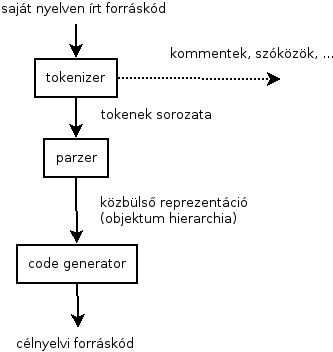
\includegraphics[scale=1]{kepek/process.png}
\caption{A keresztfordítás lépései}
\label{fig:process}
\end{figure}

\subsection{Tokenizálás}

Az tokenizálás a fordítás első lépése lesz, ebben a lépésben a felhasználó által megadott programkód beolvasásra kerül, majd a program szétbontja azt és megvizsgálja az egyes elemeket. A tokenizer minden elemhez hozzá kell tudjon rendelni a program egy tokent, így a tokenizer visszatérési értéke tokenek egy sorozata lesz.

A tokenek sorozatában nem szerepelnek a különböző fehér karakterek, mint a szóköz, újsor, tabulátor karakter, mivel a tokenizer a feldolgozás során ezeket az elemeket, mivel ezek csak az olvashatóságot növelik a kódban, a feldolgozásához, fordításhoz plusz információval nem járulnak hozzá, törli.

Ezután a többi tokent a megadott reguláris kifejezések alapján hozza létre. A leggyakoribb tokenek közül néhány példa:
szám literál: \texttt{[0-9\_]+}
szöveg literál: \texttt{[a-zA-Z0-9\_]+}
zárójelek: \texttt{(} és \texttt{)}
fehér karakterek:
\begin{verbatim}
(\\n | \\r | \\r\\n | \\f | \\t)+
\end{verbatim}

A tokenizer általában egy külön programrész, osztály a feldolgozóban, melyet általában lexernek is neveznek. Ezt az osztályt külön programok segítségével lehet megalkotni, melyeket lexer generatornak nevezik. Az interneten többféle ilyen generátor is található, melyeket segítségül hívva meg lehet alkotni a feldolgozó osztályt.

Fontos, hogy ezeknek a generátoroknak meg kell adni egy szintaktikai leírást, mely alapján a lexert létrehozzák, azonban figyelni kell arra, hogy az adott generátornak megfelelő módon, és a általunk megadott nyelvre illeszkedő kifejezéseket adjunk meg.

A fellelhető generátorok közül jelen esetben olyanok közül kell választani amelyek a reguláris kifejezések segítségével adják meg a feldolgozási elemeket. Ilyenek  például az AnnoFlex, JFlex programok, ezekről részletesebben a szintaktikai elemzés fejezetben esik szó.

A megvalósításkor nehézséget okozott a fentebb említett választás és szintaktikai leírás. Mivel a korábbi tanulmányaim során ilyenre nem került sor, a generátor általt felhasznált szintaktikai leírás megvalósítása néhány esetben hibára futott. Ami ebben segítséget jelentett, az az AnnoFlex programban megadott példa kód volt, mely alapján további reguláris kifejezéseket fel lehetett venni.

\subsection{Parser}

A tokenek sorozata ezután átkerül a feldolgozás következő lépéseként a parserhez. A parser osztályt, mely a kapott kódot feldolgozza, szintén előtte definiálni kell, melyet az adott nyelvhez kapcsolódó megadott szintaktika, illetve egy parser generator végezhet el.

A lexer generatorthoz hasonlóan a parser generator is megtalálható az interneten. Fontos megjegyezni, hogy olyan parser és lexer generatort érdemes választani, mely a lehető legjobban együtt tud műküdik. Ilyen például a JFlex és a CUP generátor, mely generátort úgy terveztek, hogy egymással együttműködve tudnak működik.

A CUP generátort emellett magában is használható egy adott token sorozat feldolgozására, ezekről részletesebben szintén a szintaktikai elemzés fejezetben esik szó.

Szintén nehézséget okozott a megfelelő parser generátor kiválasztása, hiszen annak olyannak kell lennie, hogy a kiválasztott lexer generátorral együtt tudjon működni, az az által generált eredményhalmazt be tudja olvasni. Itt is felmerültek a fájl szintaktikai megvalósításakor fellépő hibák. Sajnos a CUP parser generátor leírása nem volt annyira részletes ez ügyben, így a hibák javítása hosszabb időt vett igénybe.

\subsection{Kód generálás}

Az utolsó lépés, hogy miután a parser generator által létrehozott objektum hierarchia elkészült, ebből a program elvégzi a konvertálást, és gíy jön létre majd a célnyelvi forráskód, ami már az adott nyelv szintaktikájának megfelelő és felhasználható a programozó izlése szerint.
